\chapter{Evaluation \& Discussion}

In this chapter, I will focus on evaluating and discussing two forms of DNS abuse which are confusable domains and phishing due to their popularity among bad actors by testing and validating them,. I will delve into real-life examples to illustrate the severity of these threats and examine existing mitigations and techniques employed to mitigate them to test how well my project met the objectives. Additionally, I will propose enhancing transparency around these mitigation strategies to foster accountability and trust. Through analysis, I will assess the feasibility of implementing such transparency measures by performing analysis using the data and the evidence. Finally I will be addressing the limitations of my work. This comprehensive approach aims to provide information on addressing DNS abuse effectively while promoting transparency in the process. 


\section{Confusable Domains}
\subsection{Identification \& Examples of Targeted Domains}

The choice of such domains to target and outsource depends on many factors, each with its implications on the business strategy, marketing, and observance by law. The selection of these domains hence matters a lot in creating potential conflict especially those related to existing trademarks. Understanding these selection criteria is very important in trying to negotiate the hurdles of the digital market and in protecting rights through intellectual property. To navigate these complexities effectively, it is essential to consider several key factors. 

\begin{itemize}
  \item \textbf{Commercial Appeal:} High commercial appeal domains are lucrative targets due to the extremely high possibility of attracting a large traffic flow, with potential revenue generation and used for blackmailing purposes in which they demand payment to relinquish the domain. Such names are easy to remember, short in length, and directly linked to products or services under some category that is searched most frequently \cite{Li2002ConflictDomainTrademark}.
  
  \item \textbf{Keyword Relevance:} Targeted domains have a certain relevance that holds the keyword itself. These domains are ranked higher in search engine outputs and attract organic traffic, making them a useful tool for businesses aiming to align with the primary keywords used by their target customers in which they are targeted because they generate huge amount of clicks.
  
  \item \textbf{Similarity to Well-known Trademarks:} This refers to the practice of registering domains that are similar or confusingly like existing trademarks known as cybersquatting. This can lead to confrontations with the rightful trademark holders. Trademark law aims to prevent consumer confusion and protect the goodwill associated with the trademark, particularly in disputes over domain infringement.
\end{itemize}

\subsection{Real-life examples}

\begin{itemize}
    \item \textbf{Cybersquatting :} is securing domain names that are the same as or in the likeness of trademarks or brand names, with the intent to sell them at grossly marked-up prices back to the target , showing ads which bad actors benefit financially from clicks generated by users who visit the site expecting it to be associated with the target , harvesting emails and redirecting to malicious websites.Perhaps the best example in that respect was one of the largest dairy product companies in India, Amul. In the financial year of 2019-2020, the turnover that was brought into account through Amul was staggering, to say the least. During this period, the company was a target for cybersquatting, where some bad actors had registered similar domains impersonating as Amul. These had been used for constructing several phishing sites to further various fraudulent schemes like solicitation for payments under the pretext of distributorship of Amul products and also of securing jobs in Amul. This operation which was active between 2018 \& 2020 then finally came down to a public warning and further law actions by Amul to deal with fraudulent activities happening under these domains. Such abuses in the domain name system expose even long-established brands to threats and show the relevance of legal action and public-awareness activities for resolving them \cite{MehtaCybersquatting}.
    
    \item \textbf{Typosquatting- URL hijacking :} it deals with the registration of misspelled variants of well-known domain names for the mere purpose of capturing traffic from users who tend to make mistakes in typing a URL. They could register "goggle.com" instead of "google.com" which was used to direct users to a site that bombarded their browsers with pop-ups and ads , leading to malware infections as that site was designed to capitalise on accidental misspellings or phishing  attempts that tricked users into visiting \cite{SplunkTyposquatting}. An example in December 2020, US healthcare provider Elara Caring suffered a major cyber incident that brought into sharp perspective the vulnerabilities lying at the heart of healthcare's cybersecurity framework. The incident was initiated by gaining unauthorised computer access to email accounts of its staff and resulted in breach of personal data for more than 100,000 elderly patients. Compromised information included almost every variety of personally identifiable data, from their financial details through to Social Security numbers. The attacker, despite being detected, remained in the system for a week, which may be a signal that the incident response could be better \cite{PandaSecurityPhishing}.
    
     \item \textbf{Reverse Domain Name Hijacking  :} is the act of trademark owners trying to take a domain away from its rightful holder based on the claim of trademark rights, considering that he holds a bona fide registration over the said domain. It may otherwise be described as using legal or dispute resolution mechanisms to try to force people from their domains \cite{Sun2006DomainTrademarkConflict}.  An RDNH was claimed in a UDRP action against "groovle.com," in which the domain was purported to be too close to Google's trademark. However, since the domain was used for another search engine, it was deemed legitimately used and not to have violated Google's trademark or been registered in bad faith \cite{Singh2011ReverseDomainHijacking}.
\end{itemize}


\subsection {Homograph attacks} 

The threat of a homograph based attack weaponizing visually similar characters to swindle people persists. This is also true when attackers register domain names to appear like reputable ones, such as when the Latin letter 'l' ( lower case "el") is visually confusable with the Latin latter with 'I' ( upper case eye ), and so on. Such as http://www.paypal.com vs. http://www.paypaI.com.  Latin character homographs were traditionally used up to now, though with the advent of International Domain Names there are many more possibilities. Although this rising trend suggests a higher potential for such attacks, current data say that they are not very prevalent. Vigilance is, however, important due to the increasing trend in phishing incidents and the ease with which users can be diverted to suspicious sites.

For example, a new study measures homograph attacks on internet users: "Cutting through the Confusion" explains the growth and potential impact of such attacks \cite{holgers2006homograph}. The current study tries to measure how attackers are able to register domain names having visual similarity with respect to those which are legitimate and authoritative by using confusable characters during phishing. These confusable characters, though seemingly similar to the letters in the authoritative domains, are actually characters different from one another or come from multiple scripts like Cyrillic or Greek, represented in web browsers using punycode to maintain a consistent user experience. This study is summarised in a table of the possible confusable domain names, the count of the actual number of the confusable domain names they found available, and the authoritative domain names. For example, 'yahoo.com' has more than 5000 possible confusables but has been registered two. Another instance is 'google.com', with a thousand possible confusables yet was registered 4. These confusable domains often contain punycode in their web address, which is not immediately recognised at first glance by the average user.

This table will be added below in order to clearly show, by means of a graphic illustration, the scope and scale of homograph attacks, which point to the potential risks that these attacks could pose to online security and the awareness and mitigation strategies that need to be put in place for protecting internet users from such deceptive practices. Its noteworthy contribution will be added to the body of knowledge about how homograph attacks are leveraged and their prevalence across various high profile domains.



\captionsetup{font= footnotesize}
\begin{figure}[H]
    \centering
    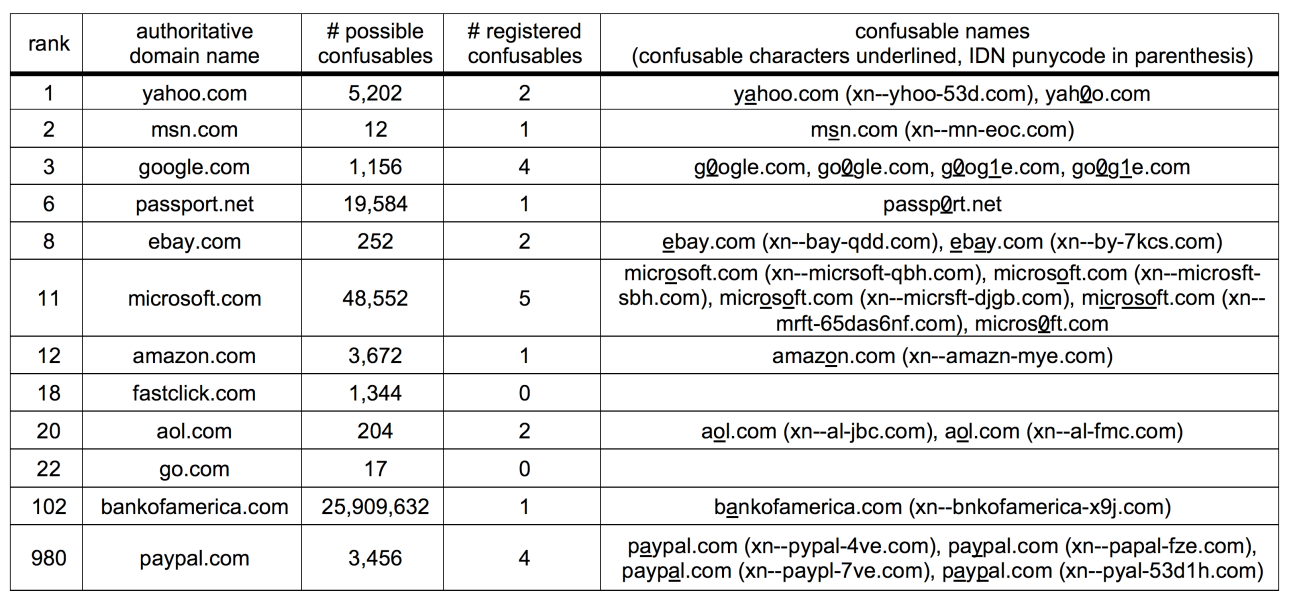
\includegraphics[width=1\linewidth]{evaluation/confusable.png}
    
    \caption{Registered confusables for popular domains, adapted from \cite{HomographAttacks}.}
    \label{fig:figureAlot1}
\end{figure}

\subsection{ Real-life Mitigations}

The following scenarios are examples of real-life confusable domain mitigations :

\begin{itemize}
    \item \textbf{Cloudflare's Zero Trust Services Approach :} Protection from this problem of newly created phishing websites is given by Cloudflare itself with its protection in the form of Zero Trust services, finding these websites, and blocking confusable domains. Cloudfare zero-trust rules can be enforced using Cloudfare Gateway in a way that they deny access to these illegitimate domains. In such a way, corporate networks are supposed to be secured from phishing attempts that take advantage of human trust in well-known brands \cite{Cloudflare2023}. Cloudflare's Zero Trust services enable a proactive approach to blocking confusable domains, which are important to avoid serving phishing sites. In particular, this mitigating measure will be triggered on the first query that involves any domain that is made through the 1.1.1.1 DNS resolver. Such queries will be inspected by the system and checked against a list of possible phishing domains through a “fuzzy” matching protocol. If the domain matches any of the saved patterns for legitimate brands, then Cloudflare's service would throw an alert. This method used by the server ensures that any domain trying to impersonate a known or respectable brand is detected as soon as it happens in which it provides both real-time monitoring and the capability to search into a historical archive of those domain names, by notifying a security team about new domains observed during the last 30 days that match their saved patterns. This enables a direct review and instant additional taking actions by this domain. The system can also be used by Cloudflare for a special investigation in a one-time domain search for some specific domain or pattern, which might become potentially dangerous from a security point of view.

     \item \textbf{IDN Handling of Google Chrome: } Google Chrome enforces an IDN (Internationalised Domain Names) policy to determine which form the Unicode or punycode form a domain label should be displayed in. The domain label is tested to determine whether it has mixed script, invisible characters, or visually confusable characters, and whether it is actually validly converted to Unicode. For instance, domains containing characters of different scripts, or those that are clearly identified as mixed script confusables, will be displayed in punycode, warning the users of potential deceptions. Chrome further offers comprehensive warnings to secure URLs that appear to be an imitation of already known web pages \cite{ChromiumIDN}.
     
\end{itemize}

In addition to what I mentioned above, let us look at the most popular mitigations used world-wide :

\begin{enumerate}
 
  \item Typo-squatting Detection Tool: Tools such as DNStwist and URLCrazy are used to offer organisations similar domain names so that they can either secure these domain names in advance or file litigation for the same.
  \item Anti-Phishing Working Group (APWG): It is a pool for stakeholders to share intelligence, trends, and best practices regarding phishing and similar threats associated with confusable domains in which mitigation is carried out in collaboration action between cybersecurity entities and domain registrars, as it allows sharing of threat intelligence with respect or cancelling out the holding of malicious domains.
\end{enumerate}

\subsection{Collaboration Among Registrars, Registries, and DNS Collaborators}

This collaboration should be achieved with DNS registry, registry, and collaborators. In that way, they can boost common resources and intelligence that can guide in making the internet more secure and resilient. This strictly falls within the remit of registries and registrars acting in collaboration to put in place such stringent registration policy with procedures for verification, checking against mimicking existing trademarks or even popular domain names. In this way, the collaboration can even manifest itself through the sharing of sensitive data with regard to domain abuse threats and trends. Databases and threat intelligence platforms are shared amongst stakeholders, allowing them to anticipate and avert most such perils well before they impact netizens. This collective effort will enable the formulation of standards by which to coordinate responses to confusable domain incident reports. Mitigating confusable domains demands that registrars, registries, and DNS collaborators work in a common effort. This is due to the increasing level of threats and the shared responsibility of all actors involved in the DNS ecosystem. \cite{Catania2022} To put this into perspective, here are some examples: 




\begin{enumerate}
  \item Recent changes in the contract from ICANN's contracted parties have imposed on registrars and registries new specifications to define DNS abuse, together with clear requirements for the actions to be taken by such parties immediately actionable evidence of abuse is received. This is a major step towards establishing more clarity about the roles that may be played by these different stakeholders in addressing the matter of DNS abuse and ensuring there is a common approach to redress \cite{Weinstein2023}.
  \item The community itself has approved new obligations from ICANN contract parties to further mitigate DNS abuse, demonstrating the will of the community to come together to address DNS abuse issues \cite{ICANN2023}.
  \item Efforts like NetBeacon, with the support of the DNS Abuse Institute, are being rolled out to reduce friction in reporting and mitigating DNS abuse. This service solves the current complexities and quality standards associated with the reporting of DNS abuse as it makes the work easier for the registrars, ultimately narrowing down their scope to the relevant and evidenced report as well as it underlines the need for cooperation among registrars, registries, and other DNS stakeholders. This is what is capable of saving the Internet and, at the same time, protecting the credibility and confidence of DNS \cite{NetBeacon}.
  
\end{enumerate}

Real-life examples of entities seeking to block the resolution of DNS names, especially in connection with public recursive DNS servers, frequently revolve around matters of control, filtering, or securing internet traffic with various kinds of motivation corresponding to such sectors. Some attempted these efforts at the government, corporate, and individual levels. As typical examples that pinpoint those instances, consider:

\begin{enumerate}
    \item Governmental Efforts to Block DNS Resolutions : Governments may interfere directly with DNS operation to enforce some censorship or block access to particular types of content. For instance, China uses the Great Firewall for regulation concerning access to the World Wide Web within their territory, including doing some mishandling connected with the DNS in order to block out unwanted content \cite{XuAlbert2017MediaCensorship}.
    \item Corporate and ISP DNS Filtering : DNS filtering can be deployed by companies and even ISPs in a bid to achieve enhanced online security. For instance, Heimdal Security explicates how the DNS filtering works as one of the measures for preventing their access to various harmful or inappropriate websites, since it first checks the requests for domains. If some are actually flagged, access is denied, hence maintaining both security and productivity within one's organisation. This approach is really very effective for the prevention of phishing and malware attacks because it stops the DNS requests towards the malicious sites \cite{
HeimdalDNSSecurity2023}.
    \item Ad Block DNS Services : Cloudflare discusses how DNS filtering can be used to prevent access to malicious sites and also filter what is harmful or unfit for viewing. This is done at the DNS level to prevent these sites from loading on devices. Cloudflare uses its DNS to filter part of a more prominent access control policy, which is an effort to secure company data and govern what employees will see on the network they manage \cite{CloudflareDNSFiltering2023} .   
\end{enumerate}

 On the negative side, attackers are taking advantage of DNS blocking mechanisms to perform DNS-based attacks. These include using DGAs (Domain Generation Algorithms) for malware communication, using FastFlux techniques for slip-streaming attacks, basically creating malicious newly registered domains (NRDs) that appear benign and legitimate to an outside observer, etc. All this makes it difficult to block bad content at the DNS level, which calls for quite sophisticated countermeasures.


\subsection{Techniques for Mitigating Confusable Domains}

Mitigating confusable domains requires sophisticated techniques tailored to address the unique challenges presented by both non-Internationalised Domain Names (non-IDNs) and Internationalised Domain Names (IDNs). This differentiation is significant due to the distinct nature of the threats they pose and the technical feasibility of the mitigation strategies applicable to each. The following is a detailed examination of mitigation techniques, along with discussions of the operational feasibility and potential collaboration frameworks involved.

Non-IDNs Mitigation Techniques : Strategies focus on identifying and mitigating domain squatting and typo-squatting, where attackers register domains that are typographical errors or close variants of legitimate domains to deceive users.

\begin{enumerate}
  \item Registry-Level Measures: Domain registries can implement checks to prevent the registration of domains that are similar to the existing trademarks or brand names, using algorithms to detect variations and misspellings closely resembling protected names. \cite{WTR2020} 
  \item Trademark Protection Programs: Services like the Trademark Clearinghouse (TMCH) offer mechanisms for trademark holders to protect their rights by receiving notifications when someone attempts to register a domain matching their trademark. \cite{ICANNTMCH}
  \item Automated Monitoring and Reporting: Automated systems can continuously monitor domain registrations for names that closely resemble known trademarks or brand names, enabling rapid detection and legal action against infringers. \cite{TMCH2023}
\end{enumerate}

IDNs Mitigation Techniques : The challenge with IDNs lies in the potential for homograph attacks, where attackers use characters from different scripts that appear visually like characters in the Latin script to create deceptive domains.

\begin{enumerate}
  \item Punycode Awareness and Monitoring: Web browsers and security tools convert IDNs to punycode, a representation that encodes the Unicode characters in ASCII. Awareness of punycode and monitoring for suspicious registrations can help identify potential homograph domains. \cite{SOCRadar2023}
  \item Browser-Level Defenses: Modern web browsers have implemented defences against IDN homograph attacks by displaying the punycode version of the domain or alerting users when a domain name contains characters from multiple scripts. \cite{Malwarebytes2017}
  \item Collaborative Blacklisting and Sharing of Threat Intelligence: Organisations can collaborate to share intelligence about known malicious IDNs, contributing to comprehensive blacklists that can be used by registrars, DNS providers, and end-users to block access to malicious sites. \cite{CyberThreatAlliance2023}
  
\end{enumerate}


However, ICANN plays a pivotal role in the detection of confusable domains as it detects confusable domains, especially with respect to Internationalised Domain Names (IDNs) but also it doesn't provide a direct list publication on confusable domain, just like the other gTLD registries. Instead, they tend to develop the frameworks and guidelines for managing the threats related to IDNs and name collisions. This will involve the development of protocols regarding how the processing of internationalised domain names would be done and how the impact that name collisions may possibly have on the domain name system is minimized. \cite{ICANNIDNs}

People detect on-Internationalised Domain Names (non-IDNs) and Internationalised Domain Names (IDNs) using comprehensive domain, IP, and DNS intelligence tools. Tools which can do so, such as those offered by services like the WhoisXML API, help check domain names for the presence of suspiciously similar domains that could potentially confuse or deceive consumers. An IDN deceptive score is given by means of an algorithm to such types of domains that take into account visual similarities, brand names, and TLD features to see if a domain name is being prepared for deceptive purposes. This approach has proven to be effective in academic research projects at identifying deceptive IDNs over millions of domains distributed across various top-level domains. \cite{WhoisXMLAPI}

\subsection{Technical \& Operational Feasibility}
The technical feasibility of these techniques varies. Registry-level measures and trademark protection programmes are quite effective, but require cooperation and standardisation across different legal jurisdictions. Automated monitoring is technically feasible and can be implemented on a scale but requires resources for continuous operation and legal follow-up. Browser-level defences are among the most directly impactful, protecting users at the point of access, yet they depend on browser vendors' willingness to implement and maintain these features, and collaboration frameworks play a crucial role in mitigating confusable domains. Initiatives such as the Trademark Clearinghouse (TMCH) facilitate cooperation between trademark holders and domain registries. Meanwhile, organisations such as the Anti-Phishing Working Group (APWG) and the Internet Corporation for Assigned Names and Numbers (ICANN) work toward broader solutions that encompass both non-IDNs and IDNs.

\subsection{ Transparency in Mitigation Efforts}

Transparency in the mitigation of confusable domains plays a pivotal role in the broader strategy to secure the Internet against phishing attacks, trademark infringement, and other malicious activities. This concept entails the practices adopted by domain registries and registrars in identifying potentially malicious domains that mimic or closely resemble legitimate ones, and the extent to which these entities disclose identified confusable domains to the public. One of the primary methods to improve transparency involves the publication of lists of confusable names by registries and registrars. These lists typically include domains flagged for their similarity to existing domain names, potentially infringing trademarks, or those that could be used for malicious purposes. The publication aims to alert the internet community, including businesses and end-users, about possible threats, thereby fostering a proactive approach to domain name security. Here is how transparency can be applied to each of the mitigation techniques described:

\begin{itemize}
  \item \textbf{Cloudflare's Zero Trust Services Approach: }Cloudflare's process for identifying and blocking confusable domains should be transparent to its users. This includes detailing the criteria for flagging domains as phishing sites and the mechanisms in place for users to appeal or request a review of blocked domains. By openly sharing the methodology behind their zero-trust rules and how they are applied through the Cloudflare Gateway, trust in Cloudflare's protective measures is bolstered among corporate networks.
  
  
  \item \textbf{IDN Handling of Google Chrome:} Google's approach to displaying domain names in Unicode or punycode based on their potential for deception benefits from transparency about its IDN policy. Detailed explanations of the checks performed (e.g., mixed script detection, invisible characters) and how decisions are made improve user understanding and awareness of potential threats. Furthermore, publishing information on how users can report misclassified domains or suggest improvements to the IDN policy can further empower users and foster a safer Internet environment.
  
  
  \item \textbf{Typo-squatting Detection Tools: }The effectiveness of tools like DNStwist and URLCrazy in helping organizations identify potential confusable domains relies on transparency about how these tools generate similar domain names and the criteria used for detection. Openly sharing updates, methodologies, and case studies can help organisations better understand how to use these tools proactively.
  
  \item \textbf{Collaborative Efforts and Intelligence Sharing: }The partnership between cybersecurity entities and domain registrars, as well as initiatives such as the Anti-Phishing Working Group (APWG), should prioritise transparency in their operations. This includes the sharing of methodologies for threat detection, the criteria for taking action against malicious domains, and the processes for stakeholders to contribute or access shared intelligence. Transparency in these collaborative efforts ensures that actions taken against confusable domains are fair, understood by all parties involved, and supported by a broad community of internet security stakeholders.
  
 \item \textbf{Transparency for non-IDN registries : } 

 \begin{enumerate}
  \item Registry-Level Measures: Transparency in level-registry measures becomes a necessity if trust has to be kept between registrants and domain trademark owners. They are published criteria and algorithms used to find variations and misspellings of the names submitted for protection. Making these publicly available can then ensure fairness and feedback in detecting mechanisms is therefore paved for improving them.
  \item Trademark Protection Programs: Services such as those from a Trademark Clearinghouse (TMCH) should operate with full transparency regarding the conductance of verification, matching, and notification. This can help trademark holders by demonstrating transparent guideline procedures that show both the rights of trademark holders and what needs to be done to effectively protect their brands.
  \item Automated Monitoring and Reporting: The automated monitoring systems must be built with such predefined criteria, algorithms, and thresholds that potentially support the involvement of stakeholders. It also makes sure that the brand owners are aware to what extent his trademarks are protected, and thus allows for some parameters within such services making the monitoring more successful.
\end{enumerate}
 
 \item \textbf{Transparency for IDN registries  : } 

  \begin{enumerate}
  \item Monitoring and Identifying Measures for Suspicious Punycode Registrations: All domain registrars and trademark owners, together with security professionals, must adhere to measures on suspicious punycode registrations. Publicising the details of activities carried out to monitor them propagates homographic threats through collective ideas, also in their identification and mitigation.
  \item Browser-Level Defences: A good web browser should play the most critical role in defending against IDN homograph attacks. Browsers must document, provide, and communicate their defence mechanisms in a clear and plain manner to users. For instance, they should indicate when a domain is being displayed in puny code or the scenarios under which their warnings are triggered. This can only give a user assurance if there is transparency as a rationality measure for them in such defence measures to be able to rationalize the triggering of any warning and know what action to take.
  \item Collaborative Blacklisting and Shared Threat Intelligence: Processes for the addition of domains to blacklists and criteria that determine whether a domain is to be considered malicious should be examined. Organisations that put in place an intelligence sharing regime also need to have some rules on data submission and validation and data disposal from blacklists. Transparency in these processes can best ensure that blacklisting is done fairly and accurately and allows the right of appeal, improving trust in collaborative security.
\end{enumerate}
  
  
\end{itemize}

In summary, transparency across all these mitigation techniques not only builds trust among users, developers, and organisations but also enhances the collective ability to respond to and prevent the threats posed by confusable domains.

\subsection{Benefits of Transparency }

The benefits of transparency in the context of confusable domains are multifaceted. Firstly, it promotes accountability among domain registrars and registries, encouraging them to actively participate in the detection and mitigation of confusable domains. Second, transparency acts as a deterrent to malicious actors who might otherwise exploit the anonymity afforded by a lack of public scrutiny. Third, by making such lists public, registries and registrars can empower businesses and trademark owners to take timely action to protect their brands, such as through legal mechanisms or domain purchases. Furthermore, transparency supports community-based mitigation efforts, where cybersecurity researchers and the wider community contribute to identifying and neutralising threats. This collaborative approach leverages the collective expertise of the cybersecurity community, enhancing the overall effectiveness of mitigation strategies.

\subsection{Drawbacks and Security Concerns} 

However, the publication of confusable domain lists is not without its drawbacks and security concerns. One major concern is that making such lists public could inadvertently provide a roadmap for malicious actors, highlighting potential targets for exploitation. This could lead to a situation where attackers use the information to refine their strategies, for example, by registering domains not yet identified or listed, thereby staying one step ahead of mitigation efforts. Another concern revolves around the risk of false positives, where legitimate domains are mistakenly flagged as confusable. This could harm businesses and individuals whose domain names are wrongfully listed, potentially leading to unwarranted scrutiny, legal challenges, and reputational damage. Moreover, the debate between transparency and security also touches on the effectiveness of disclosure in preventing attacks. While transparency aims to preemptively combat threats, there is an argument that the sheer volume of domain registrations and the dynamic nature of domain abuse may limit the practical utility of such lists to end-users and businesses.

\subsection{ Analysis : Feasibility \& Practical Challenges}

 \begin{enumerate}
  \item Automated Monitoring and Reporting: Feasible; Technology exists to automate monitoring, even though the refinement of algorithms to decrease false positives and negatives from human review can probably not be undertaken with existing resources.
  \item  Monitoring Punycode Registrations: Feasible; This option is feasible and will require mainly the use of existing technology and cooperation that could be initiated with little difficulty between relevant stakeholders.
  \item Blacklisting and Threat Intelligence Sharing: Moderately Feasible; Since agreement could be reached on shared platforms and protocols, but they imply strong cooperation and trust among such diverse entities, which is unlikely to be developed fast.
  \item Registry-Level Measures: Not Feasible; this would require very heavy coordination and agreement on standards across diverse jurisdictions and registries, very complex in nature and long-drawn.
  \item Trademark Protection Programs: Moderately Feasible; They are well-functioning processes under such adequate structures like TMCH and can be learnt while proceeding with experience, but likely to face legal and operational issues.
  \item  Browser-Level Defences: Not Feasible; While this is technically feasible, it seems rather infeasible soon that user practices will become uniform across all web browsers and that all users will be well trained in various security practices.
  \item Cloudflare's Zero Trust Services Approach: Feasible; since well-architected infrastructure and broad adoption have made Cloudflare zero-trust rules simple and effective to deploy, with a balance of security and operational efficiency without seismic root and branch changes.
  \item IDN Handling of Google Chrome and Browser-Level Defences: Feasible; Given that Chrome today has an enormous user base and that the groundwork for stopping homograph attacks already exists, it stands to reason that a solution is reasonably possible, meaning not too difficult, within a set timeline, and within the lifespan of any other typical software product.

  
\end{enumerate}

\section{Phishing}

\subsection{Real-life examples}

Phishing, a cybercrime in which targets are contacted by email, telephone or text message by someone posing as a legitimate institution to lure individuals into providing sensitive data, has become increasingly sophisticated. Two notable examples include :

\begin{enumerate}
    \item InterMed and Spectrum Healthcare Partners fell for a major phishing attack on 44,000 patient data. A Portland-based health care provider, InterMed, could have put the security of 33,000 protected health information (PHI) of its patients at risk due to an attack detected on September 6. Attackers were in the system from September 4 through September 10. The compilation of revealed information included and was not limited to names, dates of birth, health insurance information, and even clinical information accompanied with exposed social security numbers in some cases. In other data breached, Central Maine Orthopaedics issued a report affecting 11,308 patients within their service area by the Spector Healthcare Partners group. Obviously, unauthorised access to emails gives some glimpses about their patient names, date of birth, addresses, and clinical information. This is truly a bad reflection in the middle of an upswing of threats towards health data security, and thus, peremptory steps are required, not just in respect of strengthened security of emails, but in the deep training of support professionals in the best practices \cite{HIPAAJournal2020Phishing} .
    \item In a breathtaking cyber fraud case, both Google and Facebook were almost swindled out of nearly \$ 100 million each via increasingly advanced phishing attacks in less than two weeks. In fact, the fake emails were near-identical replicas of real invoices that had been sent by actual suppliers, such that trust and daily procedures were abused in making huge money transfers to fraudster-controlled accounts. This incident is only a portrayal of how susceptible research firms which are highly developed technologically are in the hands of social engineering and thus calling for the tightening of security measures, constant training of the employees, and verification of threats that have evolved in the cyberspace \cite{CNBC2019Phishing}.
\end{enumerate}

\subsection{Real-life Mitigations} 

\begin{itemize}
    \item \textbf{Employee Awareness \& Training :} Very affirmative in the number of ways a phishing activity is carried out, and the training programme prepared through simulation scenarios for the employees, the Chelsea Technologies employee education policy can be said to be the most significant. It is an inevitable approach, as in most cases, employees contain the credentials and knowledge that drive the breach to succeed. Bringing employees up to date on the different methods of phishing, for example, spoofs and malicious attachments, arms them well in the guarding of sensitive information \cite{DigitalGuardianPhishingPrevention}.

     \item \textbf{Comprehensive Security Measures :} LaptopMD points out that the risk of ignorant searching requires the formulation of policies that make it difficult to land on some sites. Besides this, the awareness on the phishers techniques and browsing issues by employees will greatly save them from being caught in cases of phishing \cite{DigitalGuardianPhishingPrevention}.
     
     \item \textbf{Technological \& Human Factors :} Each SecureHIM security approach comes with layers of added security in between these, from technological tools such as spam filters and two-factor authentication to staff. It identifies the suspicious link, abstains from clicking on it, and maybe even some browser add-ons that allow one to easily skip some dangerous links. This underscores the fact that technological peripherals and informed employees are crucially needed to provide an effective defence against phishing attacks \cite{DigitalGuardianPhishingPrevention}.

     \item \textbf{Awareness against unsolicited emails :} The Center for Democracy and Technology (CDT) outlines some of the best practices in the recognition and act to mitigate phishing; they include the sense of making urgent and unsolicited emails with poor headers, poor links, refusing to reply, open or to click on anything. The next emphasis is to train users on the awareness of phishing by setting avenues for reporting all suspicious messages \cite{CDTPhishingMitigation}.
     
     
\end{itemize}

\subsection{Techniques for Mitigating Phishing}

Current phishing attack mitigation techniques focus mainly on preventing phishing
emails from reaching the users’ inboxes and on discouraging users from accessing
phishing websites \cite{Suzuki2021Phishing}.

\begin{enumerate}
    \item Email Filters: Advanced algorithms are used to identify phishing emails based on a predetermined set of attributes, such as the reputation of the sender, links embedded in the body of the email, and keywords flagged as associated with phishing are prevented from reaching the inbox.
    \item Domain blocking: The first step at an organisational level to make the phishing site not openable by users accidentally is applying domain-blocking measures whether access to the known phishing website from inside an organisation network, this usually inhibits access.
    \item User Training: It is important that users are trained directly and reminded of any danger they are facing. Training users will require development along the lines of sensing signs in phishing emails, risk taking such as clicking on unknown links, or giving away personal or sensitive information.
\end{enumerate}

The introduction of Situational Crime Prevention Approach (SCP) \cite{Suzuki2021Phishing}, which is an idea about understanding the detailed offender thought process and the attributes in the environment allowing the attack. This approach seeks to deter potential attackers simply by raising the level of effort and risk involved in an attacker conducting a successful phishing attack with a concomitant reduction in the likely rewards. This method underscores the importance of understanding the criminal's perspective and creating a hostile environment for phishing activities through strategic preventive measures. This method involves these steps : 

\begin{enumerate}
    \item Increasing the Effort for Attackers: Implementing strong authentication methods and encryption to make it more challenging for phishers to access or spoof legitimate websites or email accounts.
    \item Clarifying User Responsibilities: Educating users about their role in maintaining cybersecurity, including recognising phishing attempts, and reporting them.
    \item Enhancing Detection Probability: Using advanced detection technologies and threat intelligence to identify and neutralise phishing threats promptly.
    \item Limiting Phishers' Access: Restrict the amount of publicly available information that could be used to create convincing phishing emails or impersonating individuals or organisations.
    \item Discouraging Future Attacks: Implementing punitive measures against identified attackers and sharing information on phishing campaigns with broader communities to prevent repeat offenders.
\end{enumerate}

This measure is designed not only to stop a phishing attack, but rather to create an environment that would lead to the cost-benefit ratio for phishing not so appealing to the attackers. In fact, comprehensive perspectives on addressing phish through the three methods above singularly go to dramatically lower the vulnerability of organisations and individual persons to such acts.

In addition, Phishlimiter \cite{Chin2018PhishLimiter} , which is a new phishing detection and mitigation approach using Software-Defined Networking where it first proposes a new technique for deep packet inspection (DPI) and then leverage it with software-defined networking (SDN) to identify phishing activities through e-mail and web-based communication.This is how it works :

\begin{enumerate}
    \item Deep Packet Inspection (DPI): Analyses the data part of network packets beyond basic header information. It inspects the content of the packets for signatures and patterns associated with phishing.
    \item Store and Forward (SF) and Forward and Inspect (FI) modes: SF mode temporarily stores packets for thorough inspection before forwarding, while FI mode prioritises immediate forwarding with parallel inspection to reduce latency.
    \item Artificial Neural Network (ANN): A machine learning model that classifies network traffic to identify potential phishing activities by learning from known phishing signatures and behaviours.
    \item Dynamic adjustment of network flows: Upon detection of a threat, the system dynamically reroutes or restricts traffic to mitigate potential phishing attacks, adapting to new threats in real time.
    \item Minimal disruption to network services: Designed to ensure that the phishing mitigation process does not significantly impact network performance, ensuring smooth operation of network services even under threat detection and mitigation activities.
\end{enumerate}

\subsection{Transparency in Mitigation Efforts}

Transparency in cybersecurity, including phishing mitigation techniques, refers to how openly and clearly the methods, policies, and procedures are communicated, understood, and accessible to all stakeholders involved, particularly employees. Here is how transparency can be applied to each of the mitigation techniques described:


\begin{itemize}
    \item \textbf{Employee Awareness and Training :} 
    
    Communication: This will consist of clear informing of the employees on the kind of threat and how it could mean for the organisation and their role in these defences.
    
Accessibility: Make people aware that the repository exists, or make the resources easily available for reference. This would include an intranet site or a repository where people could easily access the trends in phishing on the latest and how to respond.

Having a clear and simple method will inspire the employees to report the false phishing attempts and express their opinions on the training program. It encourages active participation and continuous improvement of the training material.


     \item \textbf{Comprehensive Security Measures: }
     
     Policy Publishing: All available policies, notably those related to web browsing, email attachments, and the use of security tools, will be published openly to let employees know about them.
     
Justifications: The rationale behind specific policies and restrictions so that the employee will appreciate why they are being put in place does not appear to be a set of arbitrary rules.

Changes and Updates: Introduce the workforce to changes relating to security measures and how such changes are beneficial and serve as a cover against new hazards

     \item \textbf{Technological \& Human Factors: } 
     
     Tool Transparency: Clearly state the tool and the reason for its being in place for security (e.g., spam filters, two-factor authentication), and its work on subduing phishing. 
     
User Control and Visibility: Attempt to give users some form of control or visibility over the security tools through which their work could be affected. Feedback from a blocked phishing attempt could, for example, help to reinforce the training.

A Continuous Feedback Loop: Reports and discussions of not only the phishing attempts that technology catches, but also of the ones it misses, have to be actively tracked in order to keep the human element alive in cybersecurity.


     \item \textbf{Awareness against unsolicited emails:  } 
     
     Open Communication on Threats: Constant updates on new phishing techniques and any other notable attack are discussed among the industry for them to be updated.
     
Best practices: develop best practices for easy identification and to be visible on how to catch and react to phishing attacks, with graphic examples or checklists.

Development of trust: Create an environment where employees will not have any fear of revenge for reporting any insecurity that they might suspect. This can be enabled by an easily established reporting system that is anonymous.

\item \textbf{Email Filters:} 

The effectiveness of email filtering technology in mitigating phishing attempts is greatly enhanced by transparency about its operational parameters. From disclosing the details of criteria and algorithms it uses to flag warnings over phishing e-mails to such steps as analysis of the reputation of the sender, scanning any content for embedded links and spotting keywords associated with phishing so users can start to get to grips with how the system makes its decisions. Similarly, an open forum at the beginning of the report that describes how the nature of phishing threats and the evolution of filters to catch them will help users report false positives (legitimate email incorrectly classified as phishing) or false negatives (phishing attempts which get by the filter), can encourage ongoing community participation, and more importantly, help to improve the filtering effort. In an open dialogue about the changing nature of phishing threats and adaptability of the filter in both cases, it engenders trust with users.

\item \textbf{Domain Blocking:} 

As a strategy put in place to mitigate access to known instances of phishing sites from within the organisation's network, it gains in the fact that the strategy is transparent by sharing information on criteria and constant update of the blacklist that can help stakeholders understand the reasons leading to the need for access restriction. Create a well-defined mechanism or path for the informer that the site is suspected to be, one which had not been taken into the blacklist, and also a procedure to deny false blockage (like, for example, a legitimate website in case being blocked by mistake). Educating and instructing users, as well as IT professionals, will make them aware of such a measure, and they would be made part of the secure e-culture.

\item \textbf{User Training:}

In effect, this means that users are exactly informed about the content and delivery mechanisms of such phishing-focused training programmes. For example, through the inclusion of things such as the types of phishing attacks, an explanation of why certain behaviours must be conveyed-such as the risks of clicking suspicious links, and the psychological tricks of phishers as it means users can be even more informed about the exceptionally high value of the training. Inquiring about the effectiveness of the use of training sessions and what more could be included, that users would prefer to see, will help in making the programs more user-friendly. Such sharing of success stories and statistics, of how those phishing incidents are going down right after the training, are all aspects that could fuel the energy of the employees toward uninhibited engagement and watchfulness in general. Openly discussing the challenge that advanced phishing detection presents and recognising the need for continual educative awareness might really get the ball rolling in the instillation of a culture of security and shared responsibility.

\item \textbf{Situational Crime Prevention Approach (SCP):}

SCP is said to reap tremendous benefit for the transparency of the approach that would be implemented in the means and results. In contrast, through the use of the explanation of how offenders' thinking and environmental stimulation analysis of what is used to commit phishing attacks are done, the stakeholders could possibly be enlightened on the mitigation means being employed. Useful examples in a showcase format of case studies where SCP strategies were able to defend successfully by increasing the effort and risk to the attacker,attacker, and reducing the potential gain. One could also take feedback from the community on these approaches and elicit suggestions to increase deterrence. This opens up an environment involving continuous development of one's organisation in light of such strategies and other changes.

\item \textbf{Phishlimiter:}

Transparency in the use and operation of the newly developed phishing detection and mitigation system is significant towards system acceptance and useful functionality. Detailing the technique of deep packet inspection (DPI) and its integration with SDN to pinpoint phishing activities in email and web communications can demystify the technology for users. By elaborating the criteria and algorithms used to support accuracy in the detection of potential phishing attacks, the strength and reliability of such a system can easily be communicated to stakeholders. The avenue for reporting of the inaccuracies or missed attempts to fish encourages user participation in training the new system. Sharing the progress of Phishlimiter effectiveness with metrics like the number of identified and squashed attacks cements the new-worth technologies on the best ways for handling phishing. Open discussions, for example, on the challenges experienced and in what direction Phishlimiter development has to go, invite greater support from the cybersecurity community to participate in collaboration.

\end{itemize}

\subsection{ Analysis : Feasibility \& Practical Challenges }

\begin{enumerate}
    \item Employee Awareness and Training : Feasible; Regular training and simulation exercises can be implemented across organisations of any size with scalable online platforms, requiring minimal resources beyond the initial setup.
    \item Comprehensive Security Measures :Feasible; The deployment of web filters and secure browsing policies is technically straightforward with existing technology. The main effort lies in continuous policy update and employee education.
    \item Technological and Human Factors: Feasible; The integration of spam filters, two-factor authentication, and secure browsing add-ons is readily achievable with current technology. The human element—ongoing employee vigilance—enhances the effectiveness of these tools without significant additional costs.
    \item Awareness against unsolicited emails: Feasible; Establishing and communicating best practices for handling suspicious emails involves minimal costs and leverages existing communication channels within organisations.

     \item User Training: Feasible; In fact, many of the details about training programmes based on phishing, e.g. information on how content about different methods of phishing, types of attacks, reasons why it is better to look out for who is emailing you, etc., properly belong into our reality. E.g., asking for feedback on how effective is a training program and getting recommended by customers on how to enhance them to make such programs even more user-friendly. Success stories shared and statistics after gamified training sessions motivate and inform. The test is to produce attractive and actual content and to support the process of participation, but it does not seem something excessive.
     
     \item Situational Crime Prevention Approach (SCP): Feasible;  SCP approach share insights into the thinking of the offenders as well as into the environmental facilitators to attacks. Offering case studies showing successful impacts of the SCP strategies on deterring of phishing through increased risk and efforts by the attackers can be done. However, sharing in detail the analysis of the offender behaviour may require cautious handling to avoid a 'how-to' guide for potential attackers. Engaging the community for feedback and suggestions is feasible and can foster a continuous improvement environment.
     
     \item Domain Blocking: Moderately Feasible; It is an operational overhead to keep updating blacklists and managing appeals in cases of wrongful blockages. Being able to maintain the updated blacklist and to attend to the appeals in the right manner will have an overhead for the smaller organisation or teams with little resources. Moreover, the evaluation of appeals and requests and the decision process have to be fast, so it cannot always be done with due care and proper research, but sometimes with raw speed.
     
    \item Email Filters: Not Feasible;  Although it can certainly be a good idea to describe what type of criteria and algorithms exist for the email filtering process, full disclosure may be too much, because this information will be used, no doubt by the attackers, to make a way around the filters. In fact, in case the attacker is able to fully understand how the mails are actually screened, they can alter their phishing ways to escape from the checkpoints. To some degree, transparency is possible, although full revelation of all operating parameters would represent a type of chaos where spam would just explode right through.
    
   
    \item Phishlimiter: Not Feasible; With the technical technologies as Deep Packet Inspection (DPI) and Software-Defined Networking (SDN), the complexity in Phishlimiter is at a higher level, maybe containing sensitive, proprietary security information. These three above would at best not be achieved without a fear of marking being compromised; background on the specifics of such technologies and testing on how they are integrated for phishing detection is technically too complex to summarise. Finally, the evolving and relatively complicated unpredictable tactics used by phishing attackers around the globe would demand that Phishlimiter therefore keep pace with the developments, and those making changes have to ensure that, at every point in time, it keeps up with current events, which sometimes may be difficult to disclose in real time without the adversaries having a foothold.
    
\end{enumerate}

\section{Limitations of Research Conducted on DNS Abuse Transparency }

This section lists a number of significant limitations that were observed during the research. The limitations imposed have had an effect on the extent, complexity, and applicability of the results, indicating potential avenues for future investigation to improve the understanding and efficacy of DNS abuse mitigation measures.

\begin{enumerate}
    \item Variability in reporting standards: A significant challenge encountered was the lack of uniform standards across DNS infrastructure providers, including registrars and registries, regarding the definition of abuse, the thresholds of action, and the manner in which these actions are reported. Such inconsistency has made efforts to collect and compare the data of different entities hard to piece together into one coherent picture for sensible enforcement of DNS abuse mitigation.This diversity highlights the need for standardised reporting standards by contributing to a fragmented view of abuse management procedures.

    \item Limited Availability of Data: The general lack of transparency reports that are available to the public. Many providers either don't release these reports at all or do so in a way that leaves out important information that has to be thoroughly examined. Due to the restricted breadth of research due to this data availability issue, there may be gaps in our understanding of the entire range of DNS abuse management strategies. One major obstacle to evaluating the efficacy and transparency of abuse mitigation techniques used by various parties is the lack of data.

    \item Reluctance to Share Sensitive Information: Information provided by respondents about abuses and what they do to mitigate them. In general, concerns about privacy, security, and the potential of revealing vulnerabilities to bad actors contribute to this reluctance which leads to Limiting the capacity of researchers to perform a comprehensive analysis of DNS abuse mitigation strategies.
    
    \item Dynamic Nature of DNS Abuse: The evolving tactics employed by those who abuse DNS are constantly changing, so results can be out of date very fast. It is more difficult to create best practices that are applicable and efficient over time due to this quick change. Because DNS abuse is dynamic, it requires ongoing research and strategy adaption to keep ahead of new threats.

    \item Potential Bias in Self-Reported Data: Self-reporting in transparency reports can still bias the results. Organisations have a tendency to emphasise their achievements while downplaying their shortcomings or difficulties. Because of this biased reporting, opinions about how well DNS abuse is being controlled may be distorted, which could cause mitigation efforts to be overestimated.
    
    \item Complexity of Measuring Impact: The evaluation of the efficacy of DNS abuse mitigation techniques is hampered by the nature of the internet ecosystem. The evaluation procedure is further complicated by the indirect relationship that exists between specific actions taken to combat DNS abuse and larger effects, making it challenging to gauge the effectiveness of these efforts.

    \item International and Jurisdictional Challenges: Due to the international scope of the internet, different legal and regulatory frameworks in different jurisdictions have an impact on DNS abuse and how it is mitigated. These differences highlight the need for cross-border cooperation and harmonisation by adding complications to the implementation and evaluation of transparent practices on an international scale.

    \item Ethical and Privacy Considerations: Ethical issues related to data collection and analysis that may include sensitive or personally identifiable information must be addressed in research in this field. Respecting ethical and privacy standards is very important, but it can also restrict the research approaches available, further limiting the breadth and depth of the study.

    
  
\end{enumerate}

All of those limitations point to the complex difficulties in carrying out thorough research on DNS Abuse Mitigation Transparency. Teamwork, creative thinking, and a commitment to improving research techniques and methods in this developing subject will be needed to address these problems.

\section{How well did the project meet the objectives?}

In evaluating the success and impact of the research project on DNS Abuse Transparency, a key question in assessing the achievements and influence of the study on DNS Abuse Transparency is addressed. To what extent did the project fulfil its original objectives? This section seeks to systematically evaluate the project's accomplishments in relation to its objectives, taking into account the intricate domain of DNS abuse and the difficulties associated with improving transparency and management procedures. A thorough review is provided by looking at stakeholder participation, the contribution to understanding DNS abuse, the objective achievement, and the practical consequences of the results. Shortcomings are acknowledged, and recommendations for further research and development are made, recognising both the successes and the areas that still require improvement. This reflection not only demonstrates the progress gained but also the continuous path toward a DNS ecosystem that is more open, safe, and resistant to abuse.


\subsection{Objective Fulfilment}

The project's goal was to improve stakeholder awareness and transparency about DNS abuse management. Despite encountering obstacles including inconsistent reporting guidelines and restricted data access, the effort succeeded in bringing to light significant flaws in the methods used to mitigate and handle DNS abuse. It revealed the complexity and diversity of processes across various institutions, underscoring the urgent need for standardised reporting requirements.

\subsection{Impact on Understanding DNS Abuse}

Given the difficulties, the research project provided insightful information about the state of DNS abuse mitigation. It demonstrated how DNS abuse is dynamic and how quickly changing bad actor tactics require mitigation measures to be updated on a regular basis. The research highlighted gaps in current understanding and management methods by highlighting the lack of transparency reports and providers' reluctance to provide sensitive information. These discoveries can act as a starting point for the next studies and the formulation of policies.

\subsection{Stakeholder Engagement}

It was essential to interact with stakeholders such as registries, policymakers and DNS registrars. The project encouraged discussion about the need for increased sector and jurisdiction cooperation and transparency. On the other hand, it appears that there is room for improvement in the influence on stakeholder behaviours and policies, particularly in terms of encouraging more proactive engagement and teamwork in the fight against DNS abuse.

\subsection{Practical Implications}
The project's outcomes have beneficial consequences to improve the transparency of DNS abuse mitigation. If put into practice, suggestions for creating uniform reporting guidelines and improving data exchange procedures may result in more efficient and cohesive methods for mitigating DNS abuse. These recommendations provide practical next steps for stakeholders to better address the issues raised.

\subsection{Suggestions for Improvement}

Deeper insights may be obtained for next projects by focusing study questions on newly developed DNS abuse strategies and investigating more aspects of transparency. Improving methods for engaging stakeholders, perhaps by creating more inclusive forums or working together on joint research projects, could increase the scope and quality of information gathered. Furthermore, promoting the idea of the project could lead to more noticeable adjustments in practice and policy.

\subsection{Future Vision}

This research project embarked on an extensive effort to clarify the complexity of DNS abuse transparency. Considering obstacles like the dynamic nature of abuse methods and the availability of data, the effort accomplished significant achievements in highlighting important areas for development and setting the stage for upcoming breakthroughs. The initiative is an essential move towards a more transparent and uniform strategy to mitigating DNS abuse, acknowledging the contributions and the need for continued research and cooperation. To move forward, all parties involved must work together to accept the recommendations and create a more secure, safe online environment.
